\documentclass[t]{beamer}

\setlength {\marginparwidth }{2cm}
\setlength {\parskip}{0cm}
\usepackage{todonotes}
\usepackage{siunitx}
\usepackage{subcaption}
\usepackage{apacite}    % Use APA Citation
\presetkeys{todonotes}{inline}{}
\beamertemplatenavigationsymbolsempty
\usefonttheme[onlymath]{serif}

\usepackage{algpseudocode}
\usepackage{enumitem,amssymb, yfonts, bm}
\newlist{todolist}{itemize}{2}
\setlist[todolist]{label=$\square$}
\usepackage{pifont}
\newcommand{\cmark}{\ding{51}}%
\newcommand{\xmark}{\ding{55}}%
\newcommand{\done}{\rlap{$\square$}{\raisebox{2pt}{\large\hspace{1pt}\cmark}}%
\hspace{-2.5pt}}

% \usetheme{AnnArbor}
% \usetheme{Antibes}
% \usetheme{Bergen}
% \usetheme{Berkeley}https://www.sharelatex.com/project/5b12e1a4f84b363f6f336dab
% \usetheme{Berlin}
% \usetheme{Boadilla}
% \usetheme{boxes}
\usetheme{CambridgeUS}
% \usetheme{Copenhagen}
%\usetheme{Darmstadt}
% \usetheme{default}
%\usetheme{Frankfurt}
%\usetheme{Goettingen}
% \usetheme{Hannover}
% \usetheme{Ilmenau}
% \usetheme{JuanLesPins}
\setlength{\parskip}{10pt}

% \newcommand*\vc[1]%
% {\begin{pmatrix}#1\end{pmatrix}}

\newcommand*\vc[1]%
{\left(\begin{array}{cccc}#1\end{array}\right)}


\newcommand\eqdef{\ \mathrel{\overset{\makebox[0pt]{\mbox{\normalfont\scriptsize\rmfamily def}}}{=}}\ }


\title[Eligibility propagation]{Including STDP to eligibility propagation in multi-layer recurrent spiking neural networks.}

\author[Werner van der Veen]{Werner~van~der~Veen\\\footnotesize\texttt({w.k.van.der.veen.2@student.rug.nl})}\date{\today}

\begin{document}

\begin{frame}
    \center{
\includegraphics[width=0.5\linewidth]{rugfsehor-eps-converted-to.pdf}}
    \titlepage
\end{frame}

%======================================

\small

\section{Introduction}
\begin{frame}{Introduction -- context}
    \begin{itemize}[label=--]
      \item Biological inspiration to AI
      \item ANNs and backpropagation
      \item Deep learning\\$\rightarrow$ high energy consumption
      \item Fundamental differences between DL and biological learning
      \begin{itemize}[label=--]
        \item Continuous vs. binary communication
        \item Backpropagation/BPTT vs. learning signals
      \end{itemize}
    \end{itemize}

  \end{frame}


  \begin{frame}{Introduction -- SNNs}
    \begin{itemize}[label=--]
      \item Binary spikes $\rightarrow$ no backpropagation
      \item Good performance, but not competitive with DL
      \item Leaky integrate-and-fire (LIF) neuron

    \begin{figure}[!ht]
      \centering
      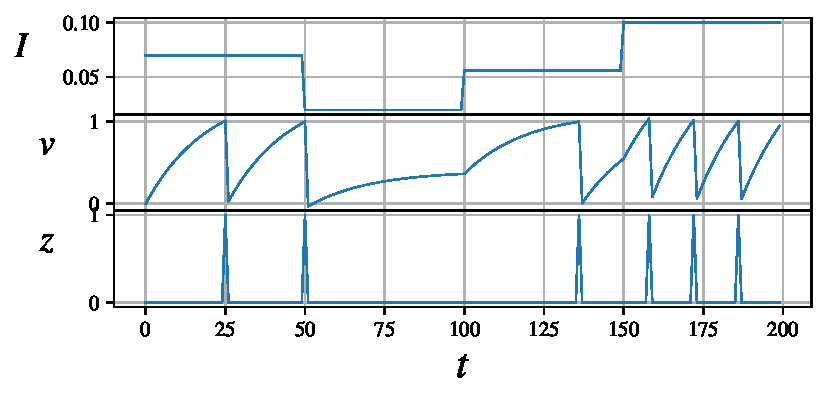
\includegraphics[width=\linewidth]{simplesnn}
    \end{figure}
    \end{itemize}
  \end{frame}

  \begin{frame}{Introduction -- neuromorphic computing}
    \begin{itemize}[label=--]
      \item Physical embedding of neural network in an analog medium
      \item Colocalized memory and computation \\$\rightarrow$ no backpropagation
      \item SNNs as ideal biologically inspired NC paradigm for efficient computation
      \item Analog SNNs are extremely fast and energy efficient
      \item Problem: learning rule must be \emph{local} and \emph{online}\\$\rightarrow$ revalue biological learning
    \end{itemize}

  \end{frame}

  \begin{frame}{Introduction -- biological learning}
    \begin{itemize}[label=--]
      \item Hebbian learning \\$\rightarrow$ runaway excitation
      \item STDP \\$\rightarrow$ how to teach?
      \item Learning signals: three-factor Hebbian learning, R-STDP
      \item Biological learning signals: neurotransmitters\\$\rightarrow$ credit assignment
      \item Eligibility traces
    \end{itemize}
  \end{frame}

  \begin{frame}{Introduction -- eligibility propagation}
    \begin{itemize}[label=--]
      \item Mathematical approximation to BPTT
      \item Local learning signals and eligibility traces
      \item Applicable to any SNN topology and multiple neuron models
      \item Also applicable to neuromorphic VLSIs
      \item Competitive with LSTMs on phone classification
      \item E-prop: only ALIF so far
      \item New research: STDP-LIF and Izhikevich neuron display STDP
    \end{itemize}
  \end{frame}

  \begin{frame}{Introduction -- this research}
  \center{Research question:\\\textit{Does including STDP-like behavior in e-prop lead to faster and more accurate phone classification?}}

    \begin{itemize}[label=--]
      \item Reproduce results of original e-prop paper
      \item Extend STDP-LIF to STDP-ALIF
      \item Experimentally verify the STDP-ALIF and Izhikevich neurons on phone classification task
    \end{itemize}
  \end{frame}


\section{Methods}
\begin{frame}{Methods -- technical framework (e-prop)}

  \begin{figure}[!ht]
    \centering
    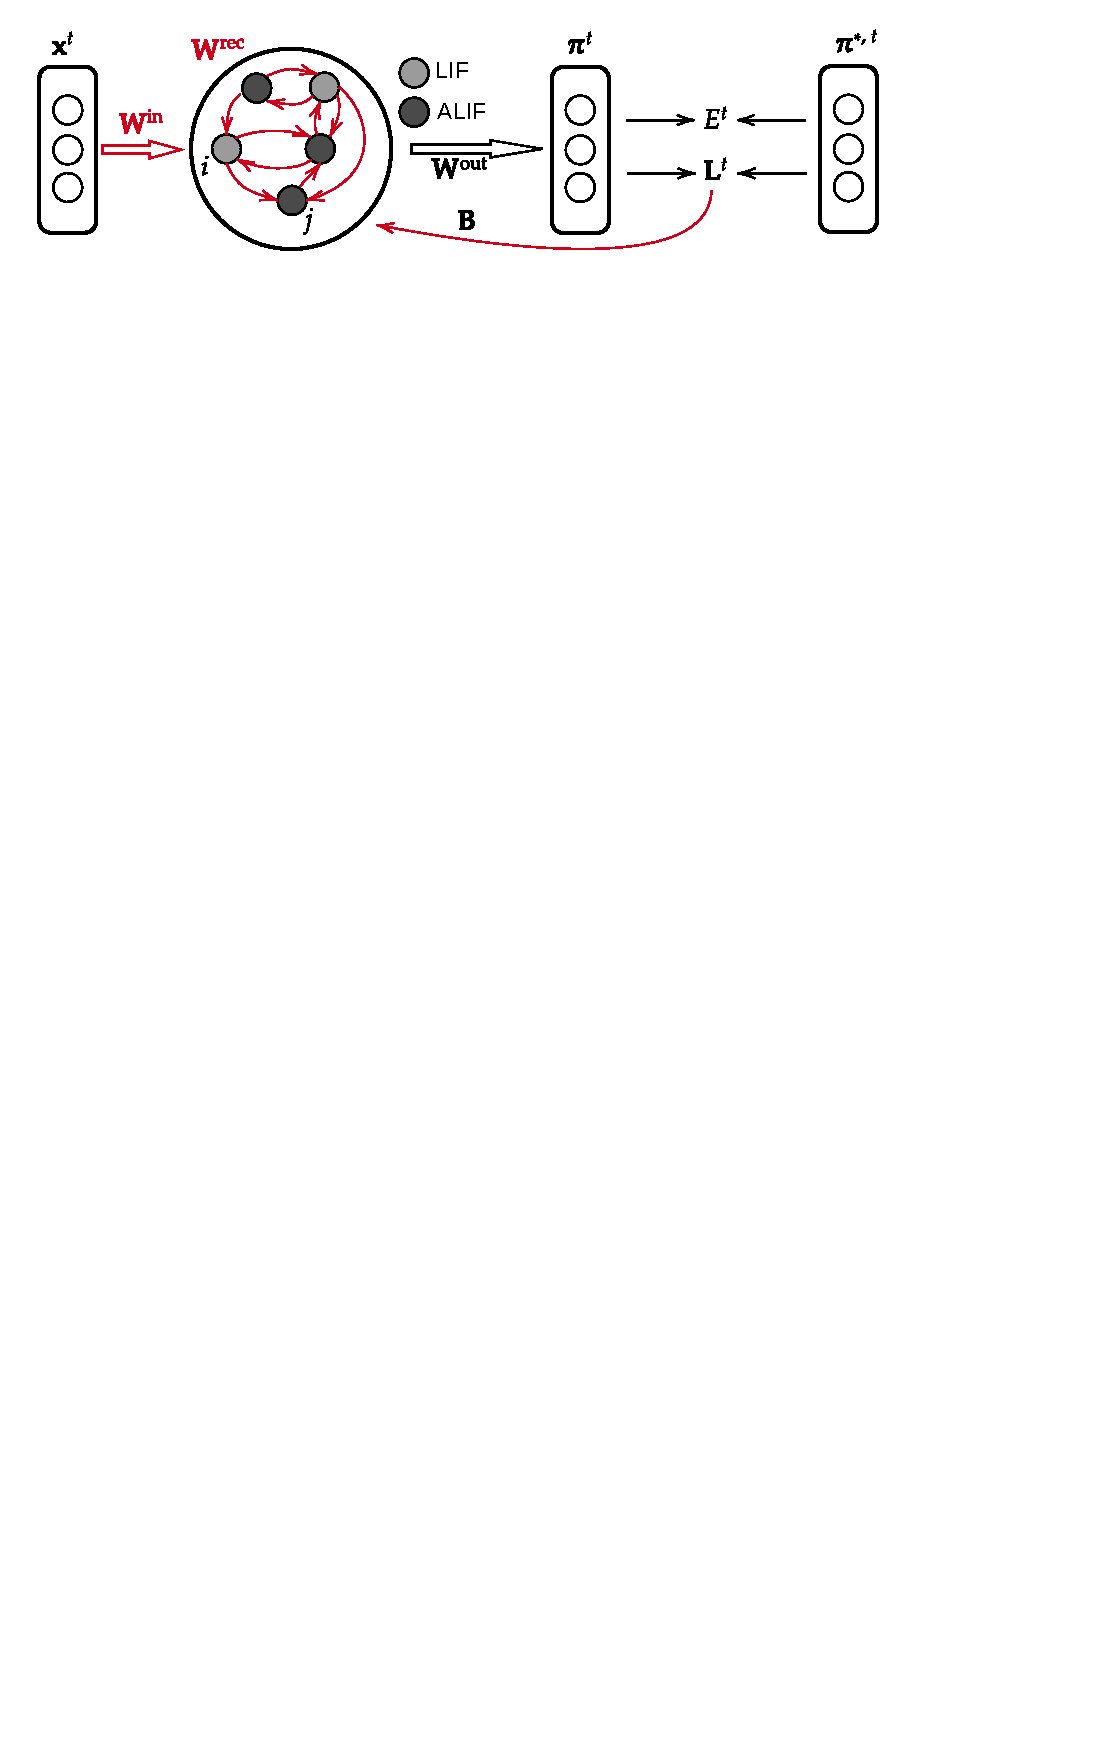
\includegraphics[trim=0 25cm 0 0, clip, width=\linewidth]{Singlelayer}
  \end{figure}
  E-prop model $\mathcal{M} = \left<M, f\right>$
  \begin{equation}\label{eq:model}
    \mathbf{h}^t_j = M\left(\mathbf{h}_j^{t-1}, \mathbf{z}^{t-1}, \mathbf{x}^t, \mathbf{W}_j\right)
  \end{equation}
  \begin{equation}
  z^t_j = f\left(\mathbf{h}_j^t\right)
  \end{equation}
  % Local and online!
\end{frame}

% \begin{frame}{Methods -- the ALIF neuron model}
%   \begin{figure}[!ht]
%     \centering
%     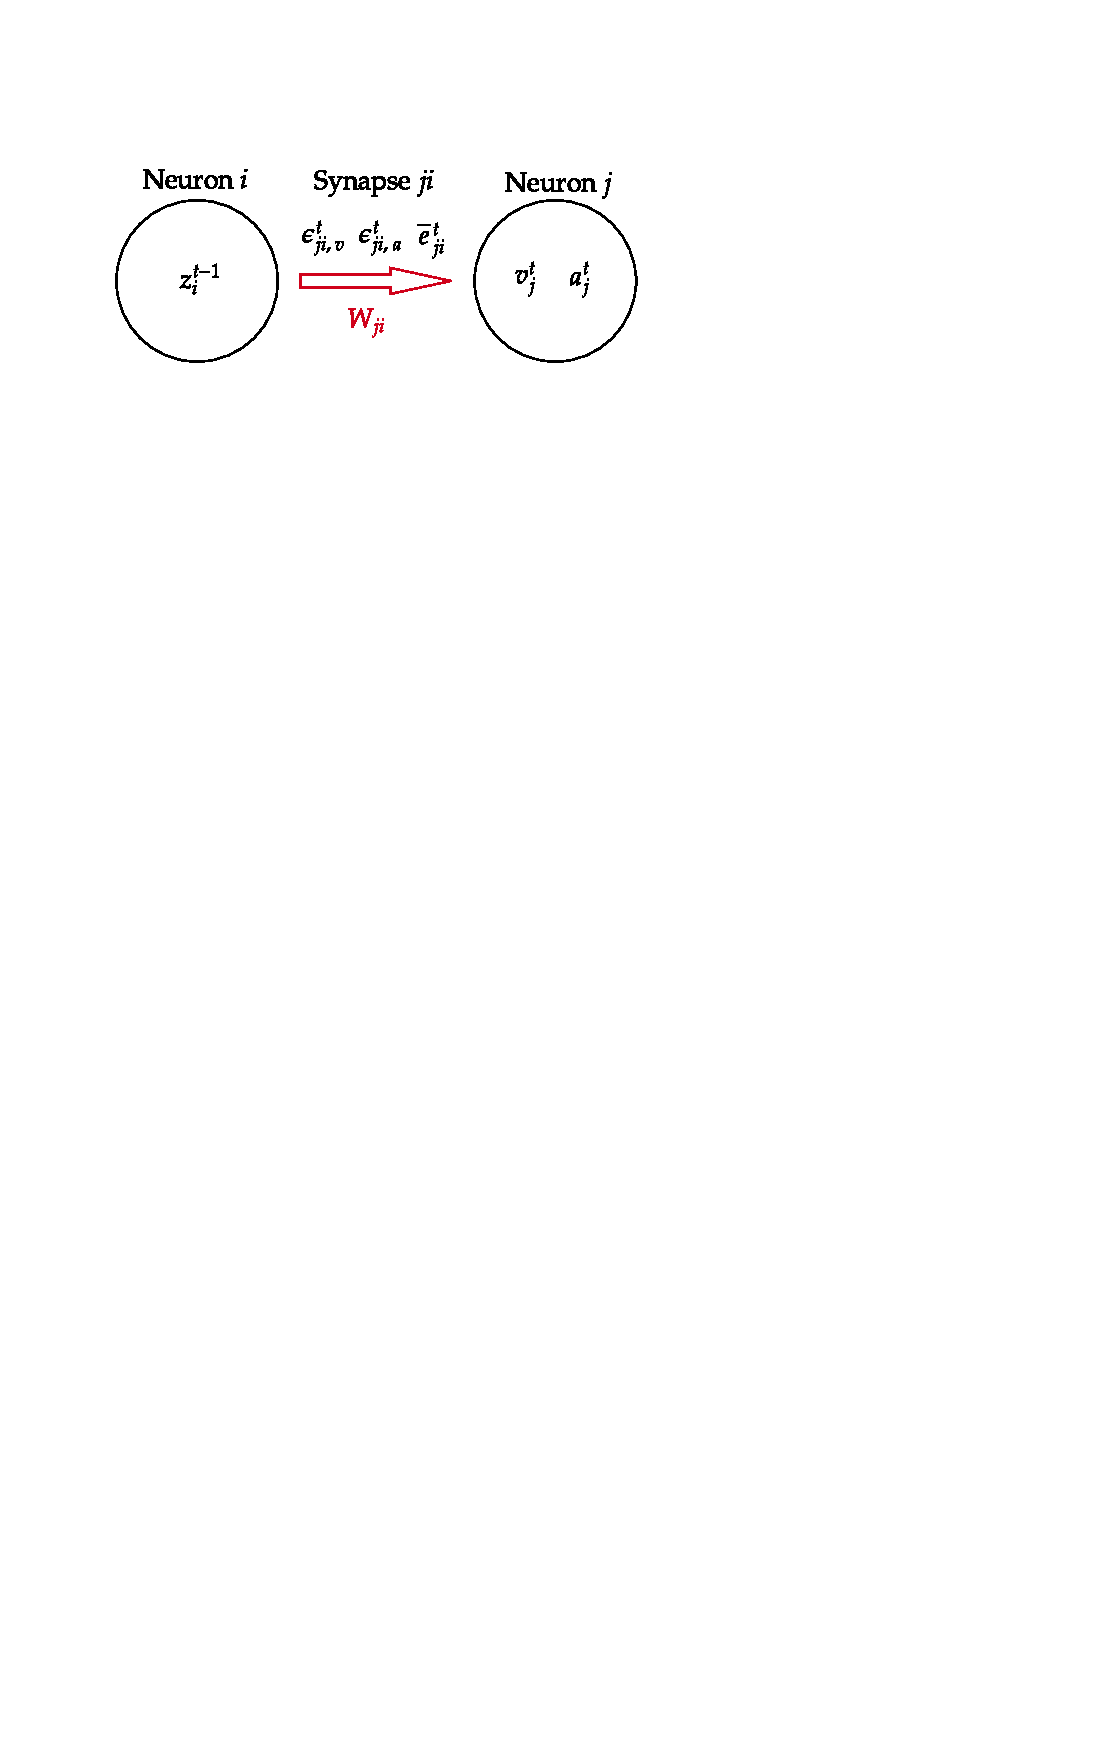
\includegraphics[width=\linewidth]{Neuron}
%   \end{figure}
%   \begin{figure}[!ht]
%     \centering
%     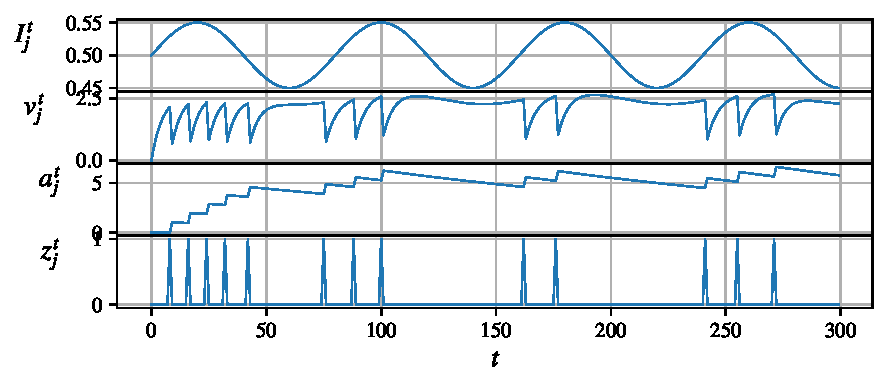
\includegraphics[width=\linewidth]{simplealif}
%   \end{figure}
% \end{frame}

\begin{frame}{Methods -- the ALIF neuron model}
  \begin{figure}[!ht]
    \centering
    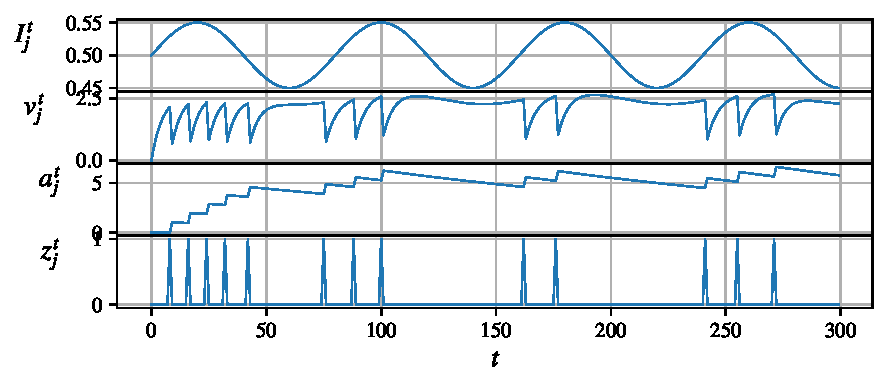
\includegraphics[width=0.9\linewidth]{simplealif}
  \end{figure}
  \footnotesize
  \begin{equation}
  z^t_j = H\left(v_j^t - v_\text{th} - \beta a^t_j\right)
  \end{equation}
  \begin{equation}\label{eq:alifV}
  v^{t+1}_j = \alpha v_j^t + \sum_{i\neq j}W^\text{rec}_{ji}z_i^t + \sum_i W^\text{in}_{ji}x_i^{t+1} - z_j^tv_
  \text{th}
  \end{equation}
  \begin{equation}\label{eq:alifA}
  a^{t+1}_j = \rho a^t_j + z^t_j
  \end{equation}
  % 25% is LIF, so effectively beta = 0
\end{frame}

\begin{frame}{Methods -- e-prop}
  \begin{align*}
    \frac{dE}{dW_{ji}} &= \sum_tL^t_j\ e^t_{ji}\\
    \frac{dE}{dW_{ji}} &= \sum_t\frac{dE}{dz_j^t}\underbrace{\frac{\partial z_j^t}{\partial\mathbf{h}_j^t}\underbrace{\sum_{t\geq t'}\frac{\partial\mathbf{h}^t_j}{\partial\mathbf{h}_j^{t-1}} \cdots \frac{\partial\mathbf{h}_j^{t+1}}{\partial\mathbf{h}_j^{t'}}\cdot\frac{\partial\mathbf{h}_j^{t'}}{\partial W_{ji}}}_{\mathbf{\epsilon}_{ji}^t}}_{e^t_{ji}}
    \end{align*}

  % pz/ph is there to make the chain rule. For LIF neurons it is the pseudoderivative, and for ALIF it is (\psi, -\beta*\psi)
\end{frame}

\begin{frame}{Methods -- e-prop for ALIF}
  Hidden state:
  \begin{equation}
  \mathbf{h}^t_j = \begin{pmatrix}
  v^t_j\\
  a^t_j
  \end{pmatrix}
  \end{equation}

  Pseudo-derivative:
  \begin{equation}
  \psi_j^t = \gamma \max\left(0, 1 - \left|\frac{v_j^t - v_\text{th} - \beta a^t_j}{v_\text{th}}\right|\right)
  \end{equation}
  Eligibility vector:
  \begin{equation}
  \begin{pmatrix}
              \epsilon_{ji, v}^{t+1}\\
              \epsilon_{ji, a}^{t+1}
              \end{pmatrix} = \begin{pmatrix}
              \alpha \cdot\epsilon_{ji, v}^t + z_i^{t-1}\\
              \psi^t_j\epsilon^t_{ji, v} + \left(\rho-\psi^t_j\beta\right)\epsilon^t_{ji, a}
              \end{pmatrix}
  \end{equation}
  Eligibility trace:
  \begin{equation}
  e^t_{ji} = \psi^t_j\left(\epsilon_{ji, v}^t - \beta\epsilon_{ji, a}^t\right)
  \end{equation}
\end{frame}

\begin{frame}{Methods -- e-prop weight update}
  \begin{equation}
    \Delta W_{ji} = -\eta\sum_t\underbrace{\sum_kB_{jk}\left(\pi^{t}_k - \pi^{*,t}_k\right)}_{=L^t_j}\underbrace{\sum_{t'\leq t}\kappa^{t'-t}e^{t'}_{ji}}_{\eqdef \bar{e}^t_{ji}}
    \end{equation}
    where $\hat{y}^t_k = \kappa \hat{y}^{t-1}_k + \sum_j W^\text{out}_{kj}z^t_j$,\\
    $y^t_k = \hat{y}^t_k+b_k$\\
    and $\pi^t_k = \sigma_k\left(y^t_1,\ldots,y^t_K\right)$.
    % Mention that output y has a low-pass filter with factor kappa.
    \begin{equation}
    \Delta W^\text{out}_{kj} = -\eta \sum_t\left(\pi^t_k - \pi^{*,t}_k\right)\sum_{t'\leq t}\kappa^{t'-t}z^t_j
    \end{equation}
    \begin{equation}
    \Delta b_k = -\eta \sum_t\left(\pi^t_k - \pi^{*,t}_k\right).
    \end{equation}
\end{frame}

\begin{frame}{Methods -- Visualizing the ALIF neuron}
  \begin{figure}[!ht]
    \centering
    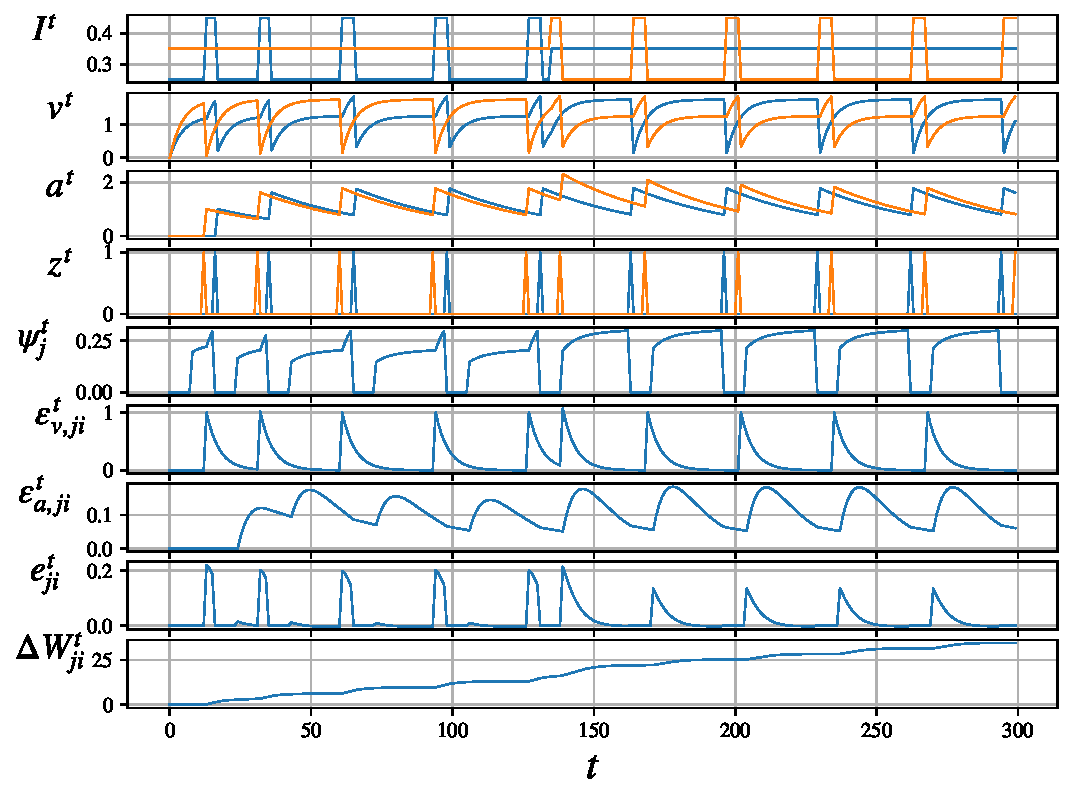
\includegraphics[width=0.8\linewidth]{alif}
  \end{figure}
\end{frame}

\begin{frame}{Methods -- STDP-ALIF}
  \begin{itemize}[label=--]
    \item New neuron model:
    \begin{align}\label{eq:ml_stdpalifV}
          v^{t+1}_{j} &= \alpha v_{j}^t + \sum_{i\neq j}W^\text{rec}_{ji}z_i^t + \sum_i W^\text{in}_{ji}I -z^t_{j}\alpha v^t_{j} - z_{j}^{t-\delta t_\text{ref}}\alpha v^t_{j}\\
          \psi^t_{j} &= \begin{cases}
          -\gamma&\mbox{if } t - t_{z_{j}} < \delta t_\text{ref}\\
          \gamma\max\left(0, 1 - \left|\frac{v^t_{j}-v_\text{th}}{v_\text{th}}\right|\right)&\mbox{otherwise}
          \end{cases}
    \end{align}
    \item Decreases $v^t_j$ after refractory period, and clamps $\psi^t_j$ to $-\gamma$ instead of to 0.
  \end{itemize}
\end{frame}

\begin{frame}{Methods -- STDP-ALIF}
  \begin{figure}[!ht]
    \centering
    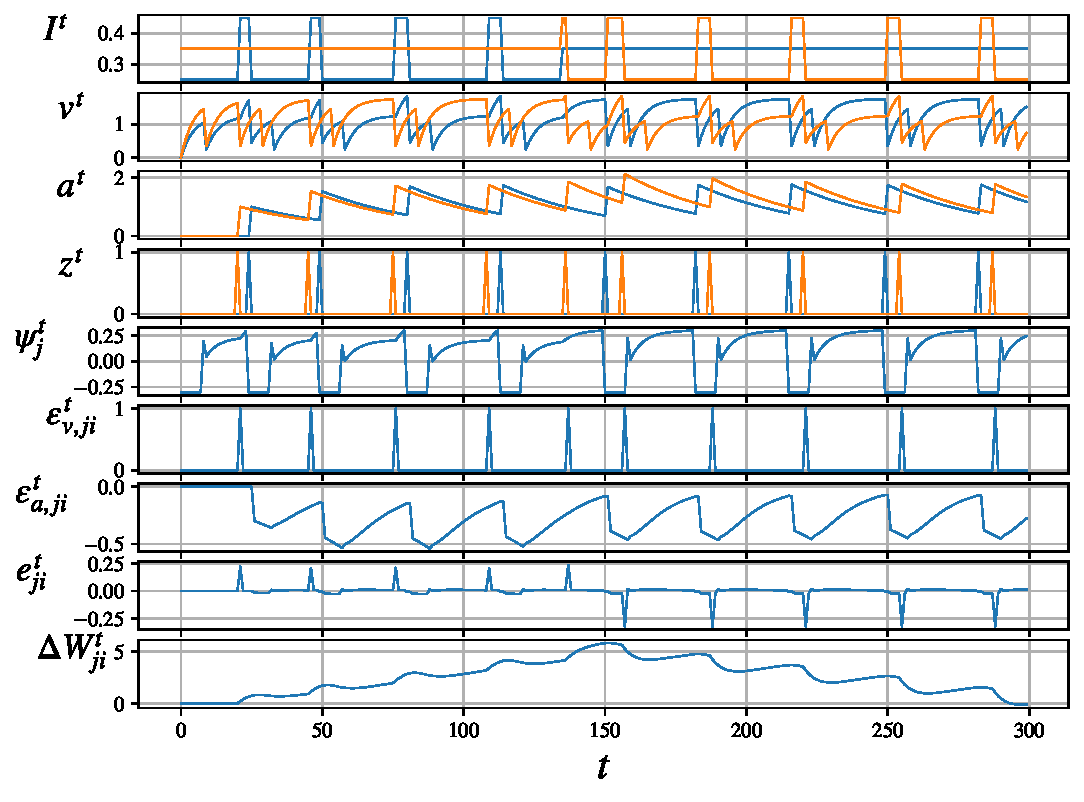
\includegraphics[width=.8\linewidth]{stdpalif}
  \end{figure}
\end{frame}


\begin{frame}{Methods -- Izhikevich}
  \begin{figure}[!ht]
    \centering
    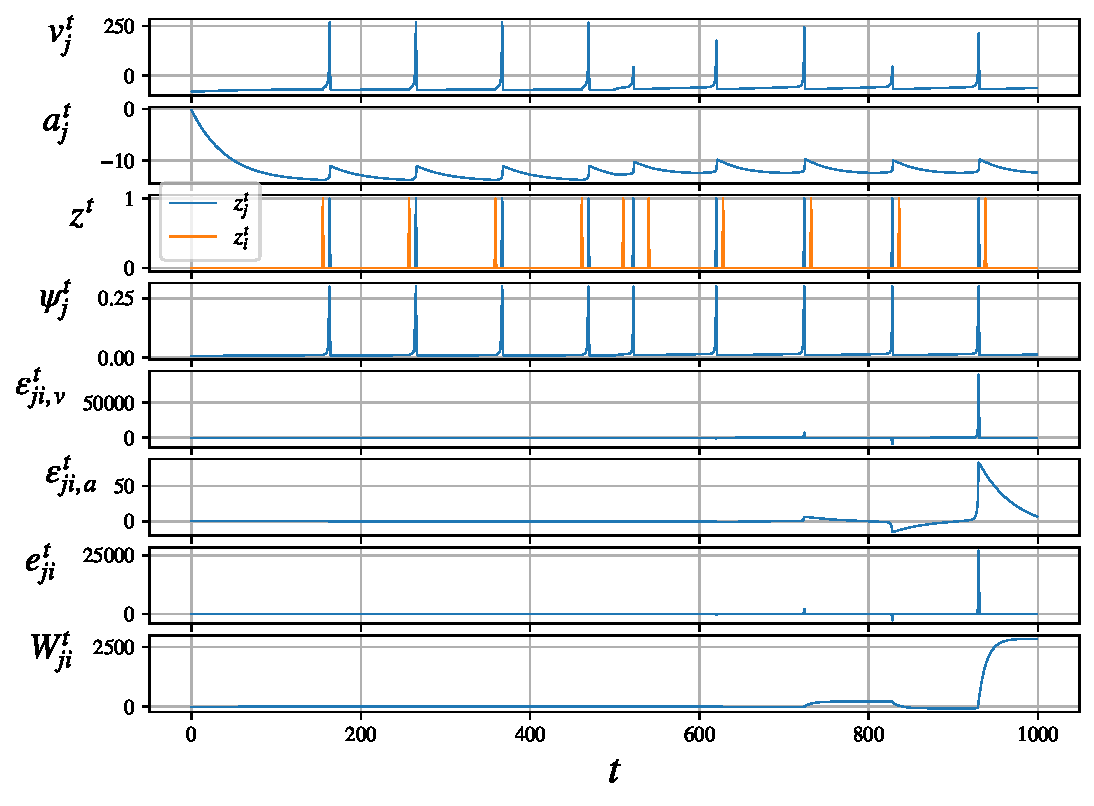
\includegraphics[width=0.8\linewidth]{demo_izh}
  \end{figure}
\end{frame}

\begin{frame}{Methods -- Izhikevich fixed}
  \begin{figure}[!ht]
    \centering
    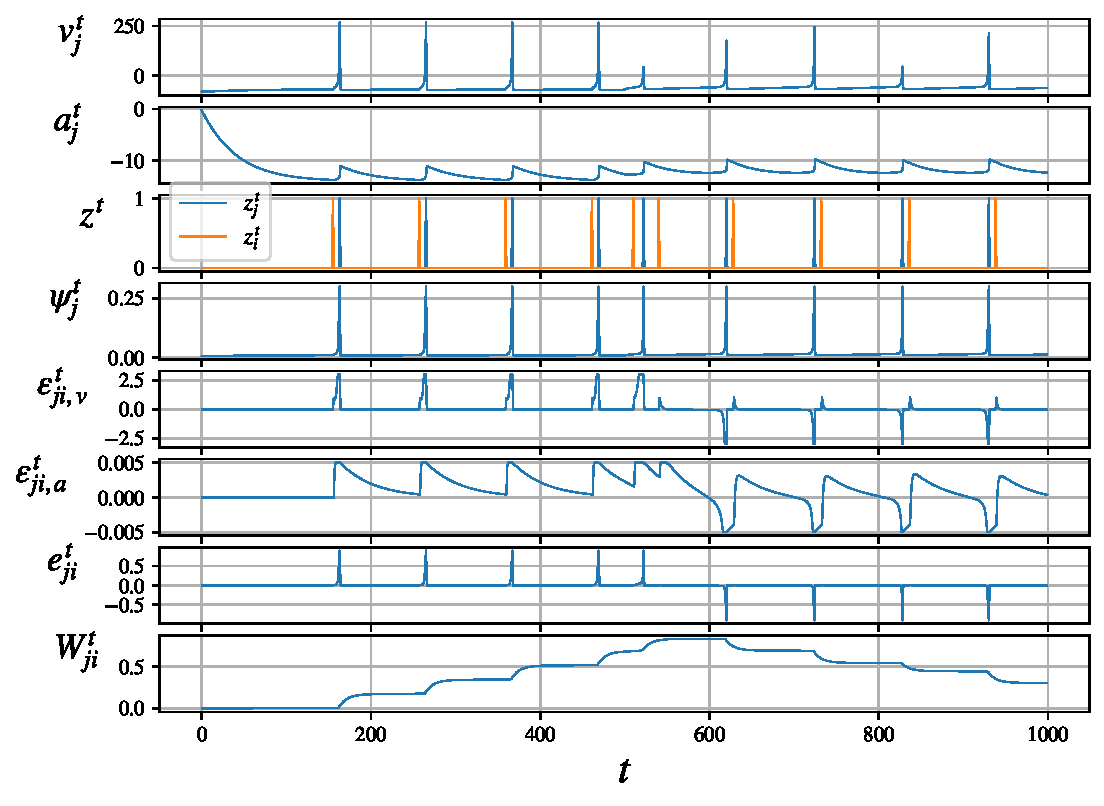
\includegraphics[width=0.8\linewidth]{demo_izh_corrected}
  \end{figure}
\end{frame}

% \begin{frame}{Methods -- Multilayer}
%   \begin{equation}\label{eq:ml_model}
%         \mathbf{h}^t_{rj} = \begin{cases}
%         M\left(\mathbf{h}_{rj}^{t-1}, \mathbf{z}_r^{t-1}, \mathbf{x}^t, \mathbf{W}_{rj}\right)       & \mbox{if } r = 1\\
%         M\left(\mathbf{h}_{rj}^{t-1}, \mathbf{z}_r^{t-1}, \mathbf{z}_{r-1}^t, \mathbf{W}_{rj}\right) & \mbox{otherwise,}
%         \end{cases}
%         \end{equation}
%         where $r \in [1\mathrel{{.}\,{.}}\nobreak R]$.

%   \begin{figure}[!ht]
%     \centering
%     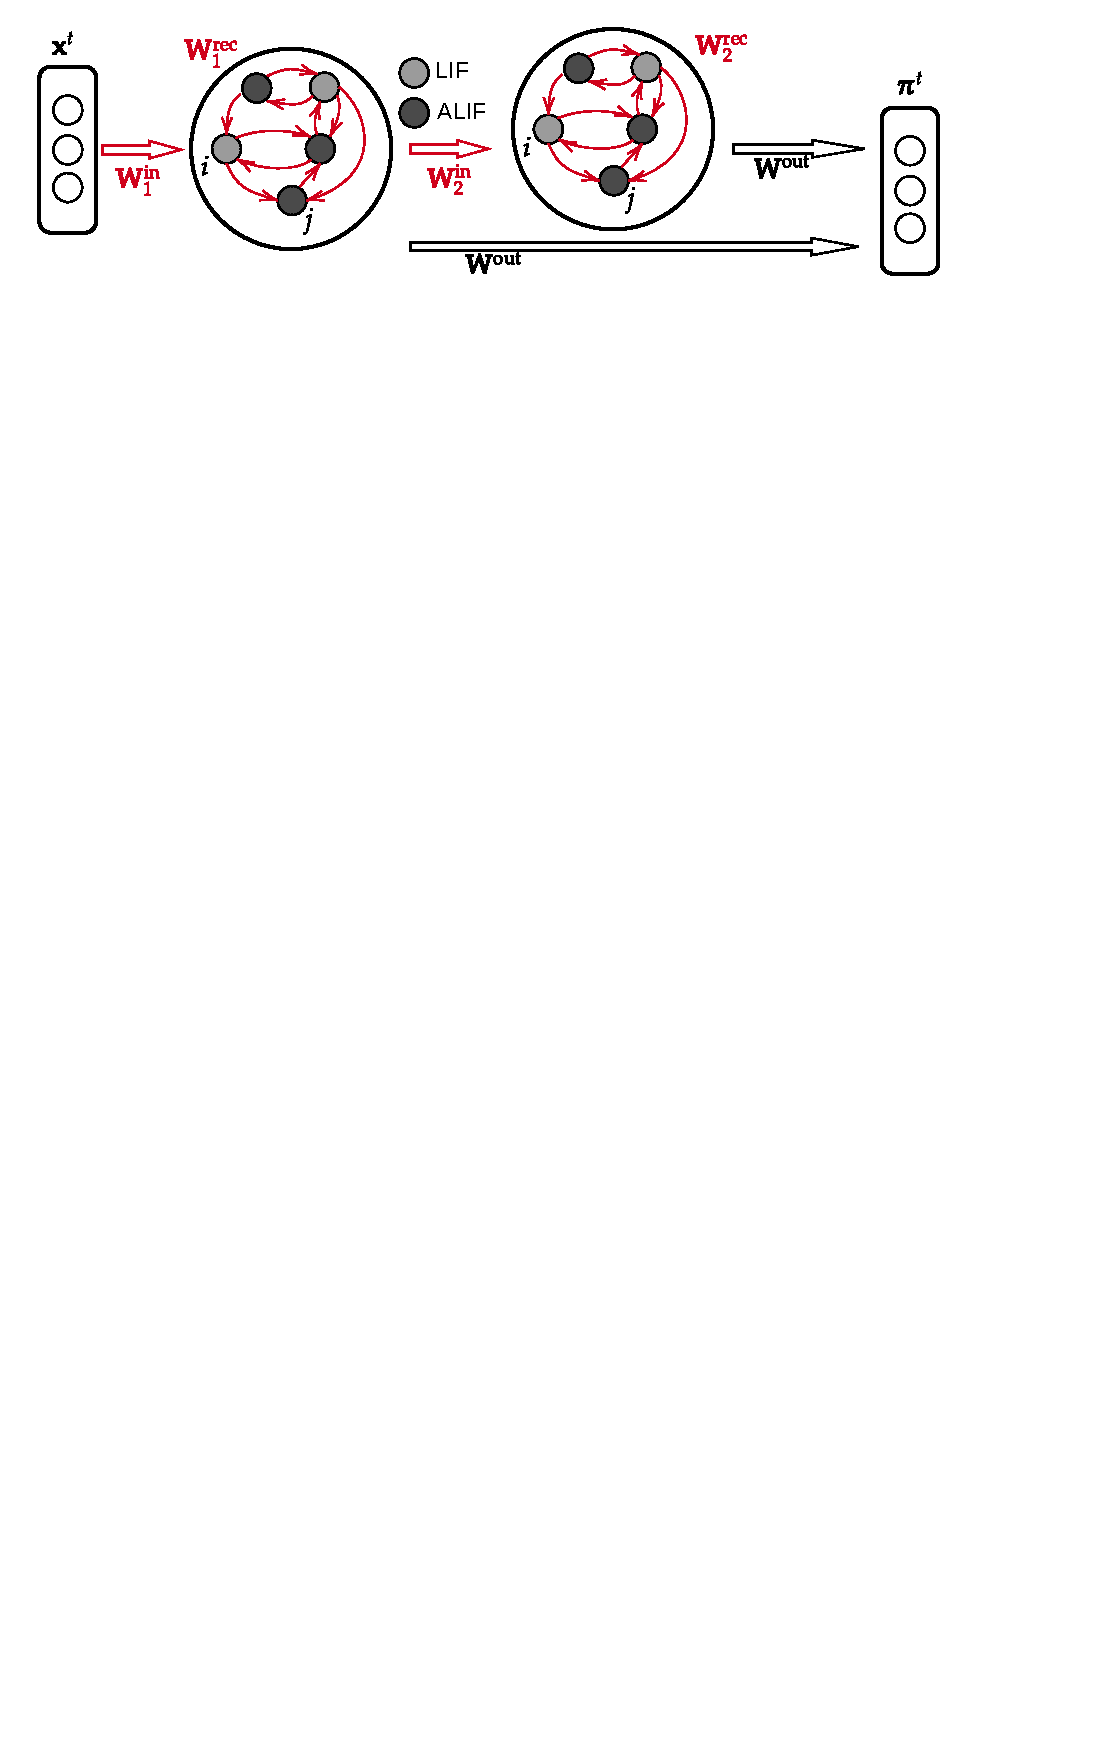
\includegraphics[trim=0 25cm 0 0, clip, width=\linewidth]{Multilayer}
%   \end{figure}
% \end{frame}

\begin{frame}{Methods -- Task}
  \begin{itemize}[label=--]
    \item Classify frame-wise phones from speech signals.
    \item There are 61 different class labels, and approximately 4000 speech sentences containing around 200-300 frames each.
    \item Speech is preprocessed into MFCCs (2--13) with their 1\textsuperscript{st} and 2\textsuperscript{nd} deltas, standardized per channel
  \end{itemize}
  \begin{figure}[!ht]
    \centering
    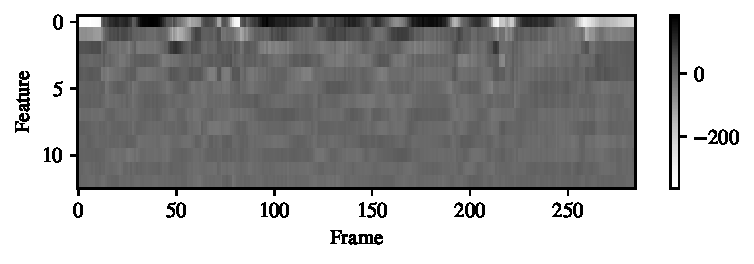
\includegraphics[width=\linewidth]{norm_mfcc}
  \end{figure}
  \begin{figure}[!ht]
    \centering
    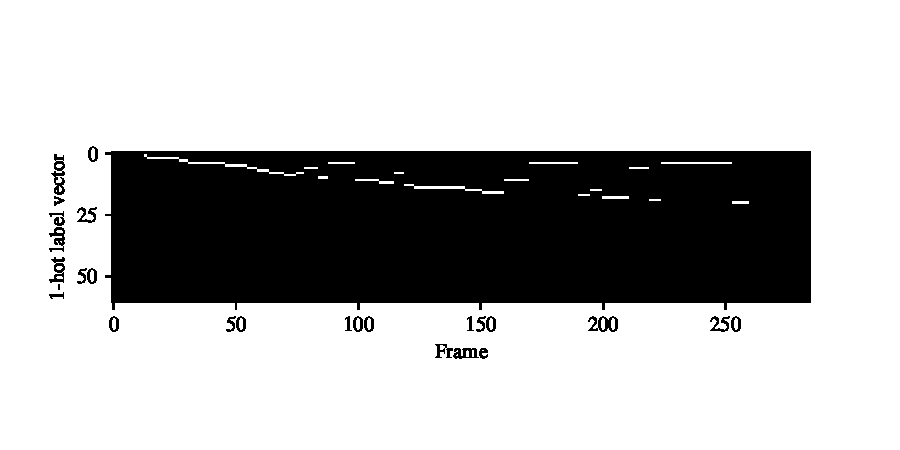
\includegraphics[width=\linewidth]{target}
  \end{figure}
\end{frame}

\begin{frame}{Methods -- Other settings}
  \begin{itemize}[label=--]
    \item Adam optimizer for e-prop
    \item Firing rate regularization
    \item L2 regularization
  \end{itemize}
\end{frame}

\section{Results}

\begin{frame}{Results -- Example}
  \begin{figure}[!ht]
    \centering
    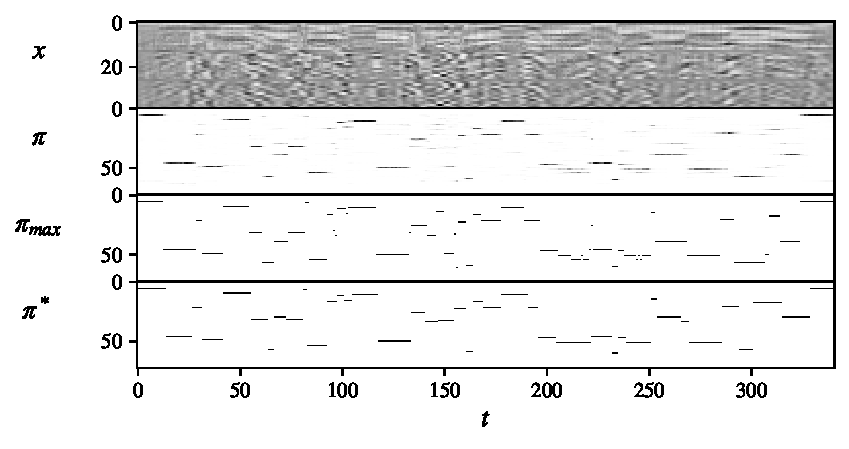
\includegraphics[width=\linewidth]{InOutPair}
  \end{figure}
\end{frame}

\begin{frame}{Results -- Accuracy per neuron type}
  \begin{figure}[!ht]
    \centering
    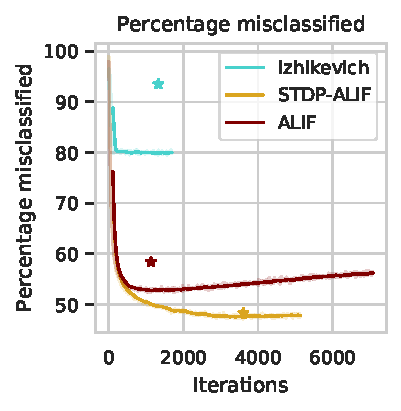
\includegraphics[width=0.5\linewidth]{percwrong}
  \end{figure}
  Test scores: ALIF = 58.4\%, STDP-ALIF = 48.3\%, Izhikevich = 93.5\%
\end{frame}

\begin{frame}{Results -- Cross-entropy per neuron type}
  \begin{figure}[!ht]
    \centering
    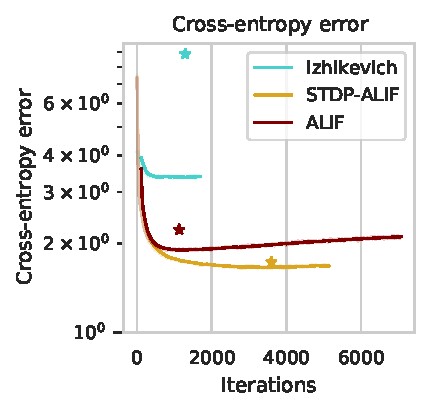
\includegraphics[width=0.6\linewidth]{crossentropy}
  \end{figure}
\end{frame}

% \begin{frame}{Results -- Multi-layer effects}
%   \begin{figure}[!ht]
%     \centering
%     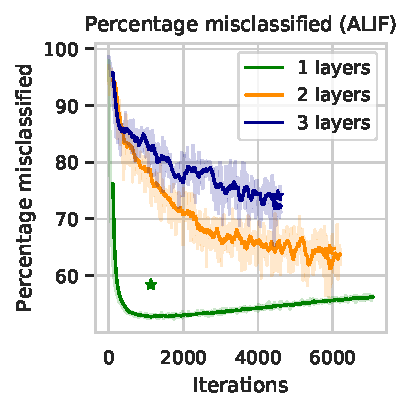
\includegraphics[width=0.6\linewidth]{ml-percwrong-ALIF}
%   \end{figure}
% \end{frame}

% \begin{frame}{Results -- Multi-layer effects}
%   \begin{figure}[!ht]
%     \centering
%     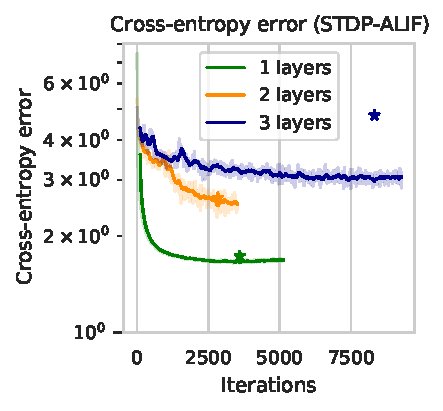
\includegraphics[width=0.6\linewidth]{ml-crossentropy-STDP-ALIF}
%   \end{figure}
% \end{frame}


\section{Discussion}
\begin{frame}{Discussion}
  \begin{itemize}[label=--]
    \item Including STDP in e-prop improves classification performance and efficiency (but not always!).\\
    $\rightarrow$ one of the best biologically plausible learning algorithms for RSNNs.
    \item Good trade-off between running cost and performance.
    \item More bioplausibility \\$\rightarrow$ easier in neuromorphic hardware but not always better performance.
    \item More research is needed on applying e-prop in other types of learning tasks, and many ideas exist that may improve performance even more.
    \end{itemize}
\end{frame}

\begin{frame}{Discussion -- future research}
  \begin{itemize}[label=--]
    \item Smoothen output
    \item Distributed parameters
    \item Custom connectivity graphs
    \item Dynamic pruning and growing
    \item Synaptic delay
  \end{itemize}
\end{frame}

\section{The end}
\begin{frame}{}
  \center{\textit{Thank you for listening!}}
\end{frame}

\section{Hidden slides}
\begin{frame}{}
  \footnotesize
  \begin{align}
  \frac{dE}{dW_{ji}} &= \sum_{t' \leq T}\frac{dE}{d\mathbf{h}_j^{t'}}\cdot\frac{\partial \mathbf{h}_j^{t'}}{\partial W_{ji}} =
  \sum_t\frac{dE}{dz_j^t}\cdot\left[\frac{dz_j^t}{dW_{ji}}\right]_\text{local}\\
  \frac{dE}{d\mathbf{h}_j^{t'}} &= \underbrace{\frac{dE}{dz_j^{t'}}}_{L^{t'}_j} \frac{\partial z_j^{t'}}{\partial\mathbf{h}_j^{t'}} + \frac{dE}{d\mathbf{h}_j^{t'+1}}\frac{\partial\mathbf{h}_j^{t'+1}}{\partial\mathbf{h}_j^{t'}}\\
  \frac{dE}{dW_{ji}} &= \sum_{t'}\left(L_j^{t'}\frac{\partial z_j^{t'}}{\partial\mathbf{h}_j^{t'}} + \left( L^{t'+1}_j \frac{\partial z_j^{t'+1}}{\partial\mathbf{h}_j^{t'+1}} + (\cdots)\frac{\partial\mathbf{h}_j^{t'+2}}{\partial\mathbf{h}_j^{t'+1}}  \right) \frac{\partial\mathbf{h}_j^{t'+1}}{\partial\mathbf{h}_j^{t'}}\right)\cdot\frac{\partial\mathbf{h}_j^{t'}}{\partial W_{ji}}\\
  \frac{dE}{dW_{ji}} &= \sum_{t'}\sum_{t\geq t'}L^t_j\frac{\partial z_j^t}{\partial\mathbf{h}_j^t}\frac{\partial\mathbf{h}^t_j}{\partial\mathbf{h}_j^{t-1}} \cdots \frac{\partial\mathbf{h}_j^{t+1}}{\partial\mathbf{h}_j^{t'}}\cdot\frac{\partial\mathbf{h}_j^{t'}}{\partial W_{ji}}\\
  \frac{dE}{dW_{ji}} &= \sum_t\frac{dE}{dz_j^t}\underbrace{\frac{\partial z_j^t}{\partial\mathbf{h}_j^t}\underbrace{\sum_{t\geq t'}\frac{\partial\mathbf{h}^t_j}{\partial\mathbf{h}_j^{t-1}} \cdots \frac{\partial\mathbf{h}_j^{t+1}}{\partial\mathbf{h}_j^{t'}}\cdot\frac{\partial\mathbf{h}_j^{t'}}{\partial W_{ji}}}_{\bm{\epsilon}_{ji}^t}}_{e^t_{ji}}
  \end{align}
\end{frame}

\begin{frame}
\begin{align}
v^{t+1}_j &= \alpha v_j^t + \sum_{i\neq j}W^\text{rec}_{ji}z_i^t + \sum_i W^\text{in}_{ji}x_i^{t+1} - z_j^tv_
            \text{th}\\
a^{t+1}_j &= \rho a^t_j + z^t_j\\
z^t_j &= H\left(v_j^t - v_\text{th} - \beta a^t_j\right)\\
\frac{\partial v_j^{t+1}}{\partial v_j^t} &= \alpha\\
\frac{\partial v_j^{t+1}}{\partial a_j^t} &= 0\\
\frac{\partial a_j^{t+1}}{\partial v_j^t} &= \psi^t_j\\
\frac{\partial a_j^{t+1}}{\partial a_j^t} &= \rho - \psi^t_j\beta\\
\frac{\partial z^t_j}{\partial\mathbf{h}^t_j} &= \begin{pmatrix}
                    \frac{\partial z^t_j}{\partial v^t_j}\\
                    \frac{\partial z^t_j}{\partial a^t_j}
                    \end{pmatrix}
                = \begin{pmatrix}
                    \psi^t_j\\
                    -\beta\psi^t_j
                    \end{pmatrix}
\end{align}
\end{frame}

\end{document}


TODO:

Include proof of e-prop on hidden slides.

Re-read own paper to refresh memory.

Write out sample text of remainder of slides, in order to streamline and focus.
